\documentclass[12pt,a4paper]{article}
\usepackage[utf8]{inputenc}
\usepackage[utf8]{vietnam}
\usepackage{amsmath,amsfonts,amssymb}
\usepackage{type1cm}
\usepackage{graphicx}
\usepackage{subfig}
\graphicspath{{images/}}
\usepackage{array}
\usepackage{enumerate}
\usepackage[unicode]{hyperref}
\usepackage{indentfirst}
\usepackage[left=1.5cm,right=1.5cm,top=2cm,bottom=2cm]{geometry}
\usepackage[american,cuteinductors,smartlabels]{circuitikz}
\usetikzlibrary{arrows}
\usepackage{tikz}
\usetikzlibrary{calc,patterns,angles,quotes}
\usetikzlibrary{arrows, decorations.markings, calc, fadings, decorations.pathreplacing, patterns, decorations.pathmorphing, positioning}
\usepackage[labelfont={bf}, textfont={it}, skip=0pt]{caption}
\setlength{\belowcaptionskip}{-10pt}


\title{\textbf{Bài giải đề thi giữa kỳ\vspace{.4cm}\\Môn học Thiết kế hệ thống điện}}
\author{SVTH: Thi Minh Nhựt -- Email: thiminhnhut@gmail.com}
\date{Thời gian: \today}

\everymath{\displaystyle}
\newcommand{\unit}[1]{~#1}
\newcommand{\unitp}[1]{~\left({#1}\right)}
\newcommand{\pfm}[1]{\left({#1}\right)}

\begin{document}

\maketitle

\tableofcontents

\section{Đề bài}
	Cho đường dây ba pha có chiều dài $210 \unit{km}$, điện áp đầu nhận là $U_R = 220 \unit{kV}$, với tần số $50 \unit{Hz}$ chuyển cho đầu nhận công suất $P_R = 150 \unit{MW}$, cho hệ số công suất ở đầu nhận là $\cos_R = 0.83$ trễ. Điện trở trên mỗi pha $r_0 = 0.16 \unit{\Omega/km}$, cảm kháng trên mỗi pha $x_0 = 0.8 \unit{\Omega/km}$ và điện dẫn trên mỗi pha $b_0 = 10^{-6} \unit{\Omega^{-1}/km}$.

	\begin{enumerate}[\it 1.]
		\item \textit{Dùng sơ đồ thay thế hình $T$ để tính các thông số sau:}\label{Diagram:hinh-T}
			\begin{enumerate}[a.]
				\item Vẽ sơ đồ thay thế hình $T$.
				\item Các thông số của đường dây.
				\item Điện áp và dòng điện đầu gửi.
				\item Công suất và hệ số công suất đầu gửi.
				\item Góc lệch pha giữa đầu gửi và đầu nhận $\Delta \varphi$.
				\item Độ sụt áp $\Delta U\%$.
				\item Tổn thất trên đường dây $\Delta P$.
				\item Hiệu suất truyền tải $H$.
				\item Vẽ giản đồ vector.
			\end{enumerate}

		\item \textit{Tính lại câu \ref{Diagram:hinh-T} với sơ đồ thay thế hình $\Pi$}.
\end{enumerate}


\section{Bài giải}
\subsection{Tính toán và lựa chọn các thông số ban đầu}
	\begin{itemize}
		\item Ta có:
		\begin{align*}
			\overline{Z} & = \pfm{r_0 + j x_0}l = \pfm{0.16 +j 0.8}\times 210 = 33.6 + j 168 = 171.33 \angle 78.69^0 \unitp{\Omega}\\
			\overline{Y} & = \pfm{g_0 + j b_0}l \approx j b_0 l = j 10^{-6}\times 210 = j 2.1 \times 10^{-4} = 2.1 \times 10^{-4} \angle 90^0 \unitp{\Omega^{-1}}
		\end{align*}

		\item Chọn $\overline{V}_R = \dfrac{220}{\sqrt{3}} \angle 0^0 = 127.02 \angle 0^0 \unitp{kV} $

		\item Suy ra: $I_R = \dfrac{P_R}{\sqrt{3}V_R \cos \varphi_R} = \dfrac{150 \times 10^3} {\sqrt{3} \times 220 \times 0.83} = 0.47 \times 10^3 \unit{A} = 0.47\unitp{kA}$.

		\item Có $\cos \varphi_R = 0.83$ (trễ) $\Longrightarrow \varphi_R = 33.90^0$.

		\item Có $\varphi_R = \varphi_{V_R} - \varphi_{I_R} \Longrightarrow \varphi_{I_R} = \varphi_{V_R} - \varphi_R = 0^0 - 33.90^0 = -33.90^0$.

		\item Nên: $\overline{I}_R = 0.47 \angle -33.90^0 \unitp{kA}$.
	\end{itemize}

\subsection[Mô hình T chuẩn]{Mô hình $\mathbf{T}$ chuẩn}
	\begin{enumerate}[ \it a. ]
		\item \emph{Sơ đồ tương đường hình $T$ chuẩn:} hình \ref{Fig:mach-tuong-duong-duong-day-trung-binh-T}.
			\begin{figure}[htp]
				\begin{center}
					\begin{circuitikz}
						\draw (-1,0) to [short, *-] (0,0) to [european resistor, l_ = $16.8 \unit{\Omega}$] (2,0) to [L, l_ = $j84 \unit{\Omega}$] (4,0) to [short] (6,0) to [european resistor, l_ = $16.8 \unit{\Omega}$] (8,0) to [L, l_ = $j84 \unit{\Omega}$] (10, 0) to [short] (12, 0) to [european resistor, l_ = $Load$] (12,-4) to [short, -*] (-1,-4);
						\draw (5,0) to [C, l_=\text{$j 2.1 \times 10^{-4} \unit{\Omega}^{-1}$}] (5,-4);
						\draw (5,0) to [short, i_ = $\dot{I}_R$] (6.4,0);
						\draw (-1,0) to [short, i_ = $\dot{I}_S$] (0.3,0);
						\draw (5,-2.5) to [short, i_ = $\dot{I}_C$] (5,-4);
						\draw (0,0) to [open, l_= \text{$\dot{V}_S$}] (0,-4);
						\draw (10,0) to [open, l_= \text{$\dot{V}_R$}] (10,-4);
						\draw[<->] (0,-.2) -- (0,-3.8);
						\draw[<->] (10,-.2) -- (10,-3.8);
					\end{circuitikz}
				\end{center}
				\caption{Mạch tương đương hình $T$ cho đường dây trung bình} \label{Fig:mach-tuong-duong-duong-day-trung-binh-T}
			\end{figure}

		\item \emph{Thông số $\overline{A}, \overline{B}, \overline{C}, \overline{D}$ cho mô hình $T$ chuẩn}
			\begin{align*}
				\overline{A} & = \overline{D} = 1 + \dfrac{\overline{Y}.\overline{Z}}{2} = 1 + \dfrac{2.1 \times 10^{-4} \angle 90^0 \times 171.33 \angle 78.69^0}{2} = 0.98 \angle 0.21^0\\
				\overline{B} & = \overline{Z} \pfm{1+\dfrac{\overline{Y}.\overline{Z}}{4}} = 171.33 \angle 78.69^0 \pfm{1 + \dfrac{2.1 \times 10^{-4} \angle 90^0 \times 171.33 \angle 78.69^0}{4}} \\
				& \hspace{3.15cm}= 169.82 \angle 78.79^0 \unitp{\Omega}\\
				\overline{C} & = \overline{Y} = 2.1 \times 10^{-4} \angle 90^0 \unitp{\Omega^{-1}}
			\end{align*}

		\item \emph{Xác định điện áp đầu gửi $\overline{V}_S$ và dòng điện đầu gửi $\overline{I}_S$}
			\begin{itemize}
				\item Ta có:
					\begin{align*}
						\left[{\begin{array}{c}
							\overline{V}_S\\
							\overline{I}_S
						\end{array}}\right]
						=
						\left[{\begin{array}{cc}
							\overline{A} & \overline{B}\\
							\overline{C} & \overline{D}
						\end{array}}\right]
						\left[{\begin{array}{c}
							\overline{V}_R\\
							\overline{I}_R
						\end{array}}\right]
						=
						\left[{\begin{array}{cc}
							0.98 \angle 0.21^0 & 169.82 \angle 78.79^0\\
							2.1 \times 10^{-4} \angle 90^0 & 0.98 \angle 0.21^0
						\end{array}}\right]
						\left[{\begin{array}{c}
							127.02 \angle 0^0\\
							0.47 \angle -33.90^0
						\end{array}}\right]
					\end{align*}

				\item Điện áp đầu gửi:
					\begin{align*}
						\overline{V}_S & = \overline{A}. \overline{V}_R + \overline{B}.\overline{I}_R = 0.98 \angle 0.21^0 \times 127.02 \angle 0^0+ 169.82 \angle 78.79^0 \times 0.47 \angle -33.90^0\\
						& \hspace{3cm} = 189.72 \angle 17.42^0 \unitp{kV}
					\end{align*}

				\item Điện áp dây đầu gửi: $V_{LS} = \sqrt{3} \times V_S = \sqrt{3} \times 189.72 = 328.60 \unitp{kV}$.

				\item Dòng điện đầu gửi:
					\begin{align*}
						\overline{I}_S & = \overline{C}. \overline{V}_R + \overline{D}.\overline{I}_R = 2.1 \times 10^{-4} \angle 90^0 \times 127.02 \angle 0^0 + 0.98 \angle 0.21^0 \times 0.47 \angle -33.90^0 \\
						& \hspace{3cm}= 0.45 \angle -30.84^0 \unitp{kA}
					\end{align*}
			\end{itemize}

		\item \emph{Xác định công suất và hệ số công suất đầu gửi}
			\begin{itemize}
				\item \emph{Xác định hệ số công suất đầu gửi $\cos \varphi_S$}
					\begin{align*}
						\cos \varphi_S = \cos \pfm{\varphi_{V_s} - \varphi_{I_{s}}}= \cos \left[{17.42^0 - \pfm{-30.84^0}} \right] = \cos 48.26^0 = 0.67
					\end{align*}

				\item \emph{Xác định công suất tác dụng, phản kháng và biểu kiến ở đầu gửi $P_S, Q_S, S_S$}
					\begin{align*}
						&\overline{S}_S = 3 \overline{V}_S.\overline{I}_S^{\ast} = 3 \times 189.72 \angle 17.42^0 \times 0.45 \angle +30.84^0 = 170.51 + j191.11 \unitp{MVA}\\
						\Longrightarrow & P_S = 170.51 \unit{MW}; \quad Q_S = 191.11 \unit{MVAr}; \quad S_S = \sqrt{170.51^2 + 191.11^2} = 256.11 \unit{MVA}
					\end{align*}
			\end{itemize}

		\item \emph{Xác định góc lệch pha giữa điện áp đầu gửi và đầu nhận $\Delta \varphi_V$}
			\begin{align*}
				\Delta \varphi_V = \varphi_{V_S} - \varphi_{V_R} = 17.42^0 - 0^0 = 17.42^0
			\end{align*}

		\item \emph{Xác định độ sụt áp $\Delta U$}
			\begin{align*}
				\Delta U \%= \dfrac{V_S - V_R}{V_R} \times 100 \% = \dfrac{189.72 - 127.02}{127.02} \times 100 \% = 49.36\%
			\end{align*}

		\item \emph{Xác định tổn thất công suất $\Delta P$}
			\begin{align*}
				\Delta P = P_S - P_R = 170.51 - 150 = 20.51 \unitp{MW}
			\end{align*}

		\item \emph{Xác định hiệu suất $\eta$}
			\begin{align*}
				\eta = \dfrac{P_R}{P_S} \times 100 \% = \dfrac{150}{170.51} \times 100\% = 87.97\%
			\end{align*}

		\item \emph{Vẽ giản đồ vector:} hình \ref{Fig:gian-do-vector-hinh-T}.
			\begin{figure}[!h]
				\begin{center}
					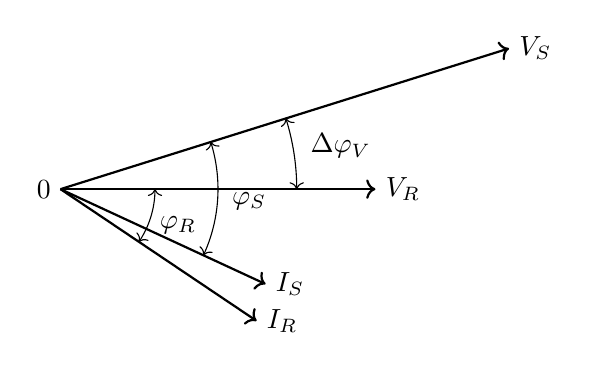
\begin{tikzpicture}
						\coordinate (origo) at (0,0);
						\coordinate (pivot) at (1,5);

						\draw (0,0) node[left] {$0$};
						\draw[thick,->] (origo) -- ++(4,0) node (VR) [right] {$V_R$};

						\draw[thick,->] (origo) -- ++(326.1:3) coordinate (IR) node[right] {$I_R$};

						\draw[thick,->] (origo) -- ++(335.16:2.87) coordinate (IS) node[right] {$I_S$};

						\draw[thick,->] (origo) -- ++(377.42:5.97) coordinate (VS) node[right] {$V_S$};

						\pic [draw, <->, "$\varphi_R$", angle eccentricity=1.3, angle radius=1.2cm] {angle = IR--origo--VR};

						\pic [draw, <->, "$\varphi_S$", angle eccentricity=1.2, angle radius=2cm] {angle = IS--origo--VS};

						\pic [draw, <->, "$\Delta \varphi_V$", angle eccentricity=1.2, angle radius=3cm] {angle = VR--origo--VS};
					\end{tikzpicture} \hspace{1cm}
					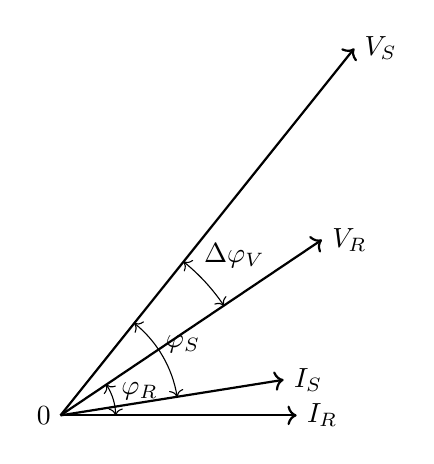
\begin{tikzpicture}
						\coordinate (origo) at (0,0);
						\coordinate (pivot) at (1,5);

						\draw (0,0) node[left] {$0$};
						\draw[thick,->] (origo) -- ++(3,0) node (IR) [right] {$I_R$};

						\draw[thick,->] (origo) -- ++(369.06:2.87) coordinate (IS) node[right] {$I_S$};

						\draw[thick,->] (origo) -- ++(393.9:4) coordinate (VR) node[right] {$V_R$};

						\draw[thick,->] (origo) -- ++(411.32:5.97) coordinate (VS) node[right] {$V_S$};

						\pic [draw, <->, "$\varphi_R$", angle eccentricity=1.5, angle radius=.7cm] {angle = IR--origo--VR};

						\pic [draw, <->, "$\varphi_S$", angle eccentricity=1.2, angle radius=1.5cm] {angle = IS--origo--VS};

						\pic [draw, <->, "$\Delta \varphi_V$", angle eccentricity=1.2, angle radius=2.5cm] {angle = VR--origo--VS};
					\end{tikzpicture}
				\end{center}
				\caption{Giản đồ vector cho mô hình T chuẩn} \label{Fig:gian-do-vector-hinh-T}
			\end{figure}
	\end{enumerate}

\newpage
\subsection{Mô hình $\Pi$ chuẩn}
	\begin{enumerate}[\it a.]
		\item \emph{Sơ đồ tương đường hình $\Pi$ chuẩn:} hình \ref{Fig:mach-tuong-duong-duong-day-trung-binh-Pi}.
			\begin{figure}[htp]
				\begin{center}
					\begin{circuitikz}
						\draw(-5,0) to [short,*-] (0,0) to [european resistor, l_ = $33.6 \unit{\Omega}$] (3,0) to [L, l_ = $j168 \unit{\Omega}$] (6,0) to [short] (8,0) to [short, i_ = $ $, l_ = \text{$\dot{I}_{R}$}] (10,0) to [european resistor, l_ = $Load$] (10,-4) to [short, -*] (-5,-4);
						\draw (6,0) to [C, l_=\text{$j1.05 \times 10^{-4} \unit{\Omega}^{-1}$}] (6,-4);
						\draw (6,-2.5) to [short, i_ = $\dot{I}_C$] (6,-4);
						\draw (0,0) to [C, l_=\text{$j1.05 \times 10^{-4} \unit{\Omega}^{-1}$}] (0,-4);
						\draw (-4,0) to [open, l_= \text{$\dot{V}_S$}] (-4,-4);
						\draw (8,0) to [open, l_= \text{$\dot{V}_R$}] (8,-4);
						\draw[<->] (-4,-.2) -- (-4,-3.8);
						\draw[<->] (8,-.2) -- (8,-3.8);
					\end{circuitikz}
				\end{center}
				\caption{Mạch tương đương hình $\Pi$ cho đường dây trung bình} \label{Fig:mach-tuong-duong-duong-day-trung-binh-Pi}
			\end{figure}

		\item \emph{Thông số $\overline{A}, \overline{B}, \overline{C}, \overline{D}$ cho mô hình $\Pi$ chuẩn}
			\begin{align*}
				\overline{A} & = \overline{D} = 1 + \dfrac{\overline{Y}.\overline{Z}}{2} = 1 + \dfrac{2.1 \times 10^{-4} \angle 90^0 \times 171.33 \angle 78.69^0}{2} = 0.98 \angle 0.21^0\\
				\overline{B} & = \overline{Z} = 171.33 \angle 78.69^0 \unitp{\Omega} \\
				\overline{C} & = \overline{Y} \pfm{1+\dfrac{\overline{Y}.\overline{Z}}{4}}= 2.1 \times 10^{-4} \angle 90^0 \pfm{1 + \dfrac{2.1 \times 10^{-4} \angle 90^0 \times 171.33 \angle 78.69^0}{4}} \\
				& = 2.08 \times 10^{-4} \angle 90.10^0\unitp{\Omega^{-1}}
			\end{align*}

		\item \emph{Xác định điện áp đầu gửi $\overline{V}_S$ và dòng điện đầu gửi $\overline{I}_S$}
			\begin{itemize}
				\item Ta có:
					\begin{align*}
						\left[{\begin{array}{c}
							\overline{V}_S\\
							\overline{I}_S
						\end{array}}\right]
						=
						\left[{\begin{array}{cc}
							\overline{A} & \overline{B}\\
							\overline{C} & \overline{D}
						\end{array}}\right]
						\left[{\begin{array}{c}
							\overline{V}_R\\
							\overline{I}_R
						\end{array}}\right]
						=
						\left[{\begin{array}{cc}
							0.98 \angle 0.21^0 & 171.33 \angle 78.69^0\\
							2.08 \times 10^{-4} \angle 90.10^0 & 0.98 \angle 0.21^0
						\end{array}}\right]
						\left[{\begin{array}{c}
							127.02 \angle 0^0\\
							0.47 \angle -33.90^0
						\end{array}}\right]
					\end{align*}

				\item Điện áp pha đầu gửi:
					\begin{align*}
						\overline{V}_S & = \overline{A}. \overline{V}_R + \overline{B}.\overline{I}_R = 0.98 \angle 0.21^0 \times 127.02 \angle 0^0 + 171.33 \angle 78.69^0 \times 0.47 \angle -33.90^0 \\
						& \hspace{3cm} = 190.42 \angle 17.48^0 \unitp{kV}
					\end{align*}

				\item Điện áp dây đầu gửi: $V_{LS} = \sqrt{3} \times V_S = \sqrt{3} \times 190.42 = 329.82 \unitp{kV}$.

				\item Dòng điện đầu gửi:
					\begin{align*}
						\overline{I}_S & = \overline{C}. \overline{V}_R + \overline{D}.\overline{I}_R= 2.08 \times 10^{-4} \angle 90.10^0 \times 127.02 \angle 0^0 + 0.98 \angle 0.21^0 \times 0.47 \angle -33.90^0 \\
						&\hspace{3cm} = 0.45 \angle -30.87^0 \unitp{kA}
					\end{align*}
			\end{itemize}

		\item \emph{Xác định góc lệch pha giữa điện áp đầu gửi và đầu nhận $\Delta \varphi_V$}
			\begin{align*}
				\Delta \varphi_V = \varphi_{V_S} - \varphi_{V_R} = 17.48^0 - 0^0= 17.48^0
			\end{align*}

		\item \emph{Xác định công suất và hệ số công suất đầu gửi}
			\begin{itemize}
				\item \emph{Xác định hệ số công suất đầu gửi $\cos \varphi_S$}
					\begin{align*}
						\cos \varphi_S = \cos \pfm{\varphi_{V_s} - \varphi_{I_{s}}}= \cos \left[{17.48^0 - \pfm{-30.87^0}} \right] = \cos 48.35^0 = 0.66
					\end{align*}

				\item \emph{Xác định công suất tác dụng, phản kháng và biểu kiến ở đầu gửi $P_S, Q_S, S_S$}
					\begin{align*}
						& \overline{S}_S = 3 \overline{V}_S.\overline{I}_S^{\ast} = 3 \times 190.42 \angle 17.48^0 \times 0.45 \angle +30.87^0 = 170.84 + j192.09 \unitp{MVA}\\
						\Longrightarrow & P_S = 170.84 \unit{MW}; \quad Q_S = 192.09 \unit{MVAr}; \quad S_S = \sqrt{170.84^2 + 192.09^2} = 257.07 \unit{MVA}
					\end{align*}
			\end{itemize}

		\item \emph{Xác định độ sụt áp $\Delta U$}
			\begin{align*}
				\Delta U \%= \dfrac{V_S - V_R}{V_R} \times 100 \% = \dfrac{190.42 - 127.02}{127.02} \times 100 \% = 49.91\%
			\end{align*}

		\item \emph{Xác định tổn thất công suất $\Delta P$}
			\begin{align*}
				\Delta P = P_S - P_R = 170.84 - 150 = 20.84 \unitp{MW}
			\end{align*}

		\item \emph{Xác định hiệu suất $\eta$}
			\begin{align*}
				\eta = \dfrac{P_R}{P_S} \times 100 \% = \dfrac{150}{170.84} \times 100\% = 87.80\%
			\end{align*}

		\item \emph{Vẽ giản đồ vector:} hình \ref{Fig:gian-do-vector-hinh-pi}

		\begin{figure}[!h]
			\begin{center}
				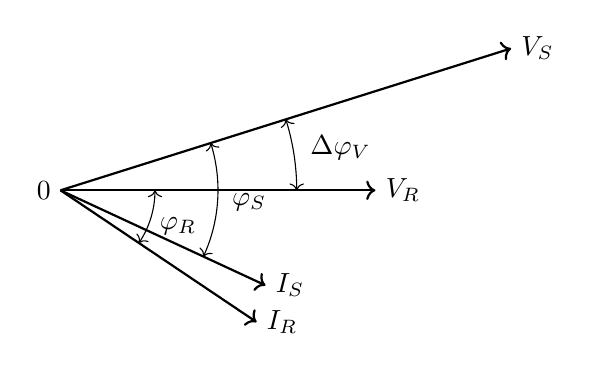
\begin{tikzpicture}
					\coordinate (origo) at (0,0);
					\coordinate (pivot) at (1,5);

					\draw (0,0) node[left] {$0$};
					\draw[thick,->] (origo) -- ++(4,0) node (VR) [right] {$V_R$};

					\draw[thick,->] (origo) -- ++(326.1:3) coordinate (IR) node[right] {$I_R$};

					\draw[thick,->] (origo) -- ++(335.13:2.87) coordinate (IS) node[right] {$I_S$};

					\draw[thick,->] (origo) -- ++(377.48:6) coordinate (VS) node[right] {$V_S$};

					\pic [draw, <->, "$\varphi_R$", angle eccentricity=1.3, angle radius=1.2cm] {angle = IR--origo--VR};

					\pic [draw, <->, "$\varphi_S$", angle eccentricity=1.2, angle radius=2cm] {angle = IS--origo--VS};

					\pic [draw, <->, "$\Delta \varphi_V$", angle eccentricity=1.2, angle radius=3cm] {angle = VR--origo--VS};
				\end{tikzpicture} \hspace{1cm}
				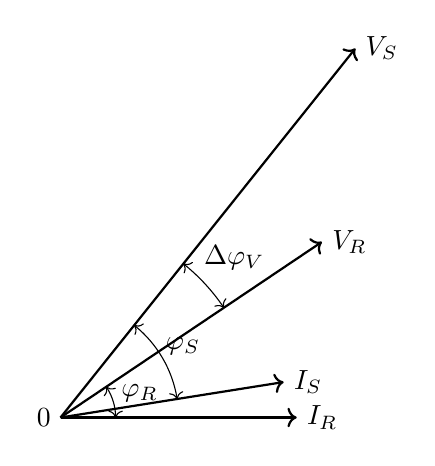
\begin{tikzpicture}
					\coordinate (origo) at (0,0);
					\coordinate (pivot) at (1,5);

					\draw (0,0) node[left] {$0$};
					\draw[thick,->] (origo) -- ++(3,0) node (IR) [right] {$I_R$};

					\draw[thick,->] (origo) -- ++(369.03:2.87) coordinate (IS) node[right] {$I_S$};

					\draw[thick,->] (origo) -- ++(393.9:4) coordinate (VR) node[right] {$V_R$};

					\draw[thick,->] (origo) -- ++(411.38:6) coordinate (VS) node[right] {$V_S$};

					\pic [draw, <->, "$\varphi_R$", angle eccentricity=1.5, angle radius=.7cm] {angle = IR--origo--VR};

					\pic [draw, <->, "$\varphi_S$", angle eccentricity=1.2, angle radius=1.5cm] {angle = IS--origo--VS};

					\pic [draw, <->, "$\Delta \varphi_V$", angle eccentricity=1.2, angle radius=2.5cm] {angle = VR--origo--VS};
				\end{tikzpicture}
			\end{center}
			\caption{Giản đồ vector cho mô hình $\Pi$ chuẩn} \label{Fig:gian-do-vector-hinh-pi}
		\end{figure}
	\end{enumerate}
\end{document}
